\documentclass{article}
% \usepackage{xeCJK}
\usepackage{amsmath}
\usepackage{amssymb}
\usepackage{mathrsfs}
\usepackage{xcolor}
\usepackage{bm}
\usepackage{hyperref}
\usepackage{graphicx}
\usepackage{subcaption}
\usepackage{float}
\usepackage{csquotes}
\usepackage{multicol}
\usepackage[ruled,linesnumbered]{algorithm2e}

\bibliographystyle{plain}
\setlength{\parindent}{2em}
\usepackage{geometry}
\geometry{a4paper, left=2.54cm, right=2.54cm, top=3.18cm, bottom=3.18cm}

% 设置文章行距
% \renewcommand{\baselinestretch}{1.5}

% define reference format
\hypersetup{
    colorlinks=true,
    linkcolor=blue,
    urlcolor=blue,
    citecolor=blue,
    linkbordercolor=white
}

\title{\textbf{Enhancement of Phase Separation in Swarmalators with Chirality-induced Frustration}}
\author{Yichen Lu}

\begin{document}

\maketitle

\tableofcontents

\newpage
\section{\label{sec:model}The Model}

Swarmalators have a spatial position $\mathbf{r}_i=\left( x_i, y_i \right)$ and an internal phase $\theta_i$ which evolve according to equations:
\begin{subequations}
    \label{eq:totalDynamics}
    \begin{align}
        \dot{\mathbf{r}}_i&=v\mathbf{p}\left( \theta _i \right)\label{eq:dotR}\;,\\
        \dot{\theta}_i&=\omega _i+K\sum_{j\in A_i}{\left[ \sin \left( \theta _j-\theta _i+\alpha _{ij} \right) -\sin \alpha _{ij} \right]}\label{eq:dotTheta}\;,
    \end{align}
\end{subequations}
\color{blue}
Mean-field definition:
\begin{subequations}
    \label{eq:totalDynamicsMeanField}
    \begin{align}
        \dot{\mathbf{r}}_i&=v\mathbf{p}\left( \theta _i \right)\label{eq:dotR}\;,\\
        \dot{\theta}_i&=\omega _i+\frac{K}{\left| A_i \right|}\sum_{j\in A_i}{\left[ \sin \left( \theta _j-\theta _i+\alpha _{ij} \right) -\sin \alpha _{ij} \right]}\label{eq:dotTheta}\;,
    \end{align}
\end{subequations}
\color{black}
for $i=1,2,\ldots,N$. Here in Eq.~(\ref{eq:dotR}), $\mathbf{p}\left( \theta \right) =\left( \cos \theta ,\sin \theta \right)$, which means each swarmalator rotates with a constant speed $v$ in the direction of its instantaneous phase $\theta_i (t)$. As per Eq.~(\ref{eq:dotTheta}), the sum runs over neighbors within a coupling radius $d_0$ around swarmalator $i$:
\begin{equation}
    A_i\left( t \right) =\left\{ j\mid \left| \mathbf{r}_i\left( t \right) -\mathbf{r}_j\left( t \right) \right|\leqslant d_0 \right\} \;,
\end{equation}
$K$ is the coupling strength, and $\omega_i$ is the natural frequency of the $i$-th swarmalator. 
This means that a swarmalator will rotate with the angular velocity $|\omega_i |$ in the absence of mutual coupling ($K=0$), and the sign of $\omega_i$ represents the direction of rotation, namely, the tribute of the chirality of the $i$-th swarmalator. A positive (negative) chirality ($\omega$) describes the counterclockwise (clockwise) rotations of the swarmalator in space. 
Here, we consider the natural frequencies of swarmalators to be distributed in a standard Lorentzian form:
\begin{equation}
    \label{eq:lorentzian}
    g\left( \omega \right) =\frac{1}{\pi}\frac{\Delta}{\omega ^2+\Delta ^2}\;,
\end{equation}
where $\Delta$ is the half-width at half-maximum of the distribution. The max density of the distribution is at $\omega=0$, and the distribution is symmetric about it, which is the most prone situation to chiral mixing.

Additionally, $\alpha_{ij}$ is the phase frustration between two neighboring swarmalators, which is defined as:
\begin{equation}
    \alpha _{ij}=\begin{cases}
        \alpha _0,&		\omega _i\omega _j<0\\
        0,&		\omega _i\omega _j\geqslant 0\\
    \end{cases}
\end{equation}
When $\alpha_0=0$, the dynamics reduces to the normal chiral model.

For simplicity, we assume that swarmalators are initially distributed uniformly in a two-dimensional $L\times L$ square with periodic boundary conditions. When two swarmalators are on opposite sides of the square, the absolute value of the difference between at least one of their coordinates is larger than $L/2$. In this case, we take the minimum distance between them, which is the relative distance between the two points in the periodic boundary conditions.

Some order parameters can be introduced to measure the level of spatiotemporal coordination among swarmalators and distinguish the different collective states of the system. Firstly, the usual order parameter to measure the chiral phase separation among swarmalators can be defined as:
\begin{equation}
    S\left( t \right) =\frac{1}{N}\sum_{i=1}^N{\frac{\sum_{j\in A_i}{H\left( \omega _i\omega _j \right)}}{\left| A_i\left( t \right) \right|}}\;,
\end{equation}
where $H\left( x \right) =\left( x>0 \right)$ is the Heaviside step function. $S\left( t \right)$ is the fraction of the pairs of neighboring swarmalators with the same chirality. When $S\left( t \right)=1$, all the neighboring pairs of swarmalators have the same chirality, and the system is in a completely phase-separated state. When $S\left( t \right)< 1$, the system is in a mixed state.

We conducted numerical simulations to investigate the performance and characteristics of our system under various conditions.
All the numerical simulations of the model Eq.~(\ref{eq:totalDynamics}) were run on Python using Euler integration with box size of $L=10$, population sizes of $N=500, 1000$ for single/double-chiral swarmalators, respectively, maximum and minimum absolute values of natural frequencies $\omega_{\max}=3$, $\omega_{\min}=1$, coupling strength $\lambda$ in $\left[ 0.01, 0.1 \right] \cup \left[ 0.1, 1 \right]$ with step length $0.1$, $0.05$, respectively, action radius of $d_0$ in $\left[ 0.1, 1 \right] \cup \left[ 1, 2 \right]$ with step length $0.05$, $0.5$, respectively, a time step $\Delta t=0.01$, and total number of iterations of $T=60000$. Unless otherwise stated, each data point of order parameters $R$, $R_c$ and $N_r$ was collected by averaging last 1000 time steps of the simulation to discard the transients.

\section{\label{sec:behaviors}Frustration-enhanced phase separation}
\begin{figure}[H]
    \centering
    \begin{subfigure}{0.45\textwidth}
        \centering
        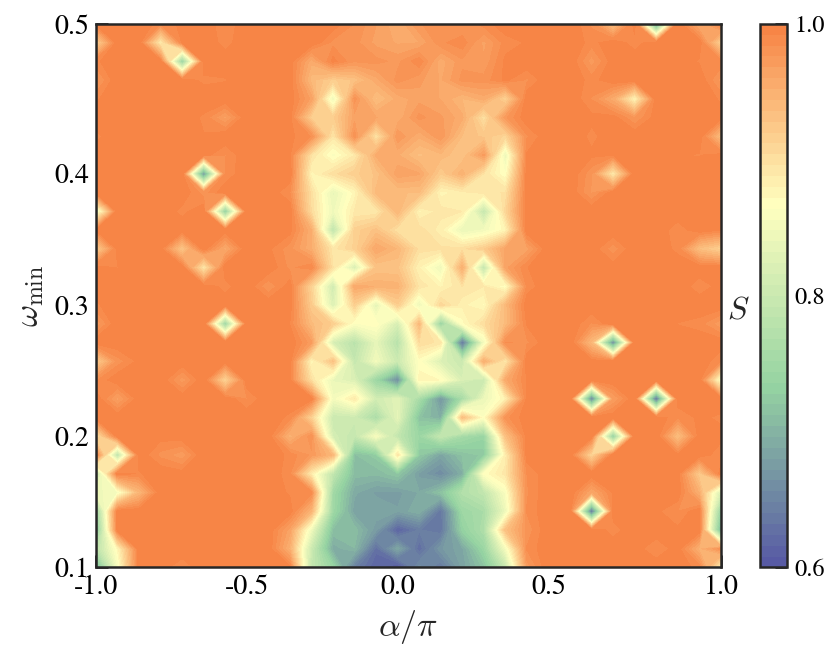
\includegraphics[width=1\textwidth]{figs/pd1.png}
        \caption{$\Delta \omega=1$}
        \label{fig:phaseDiagramDeltaOmega1}
    \end{subfigure}
    \begin{subfigure}{0.45\textwidth}
        \centering
        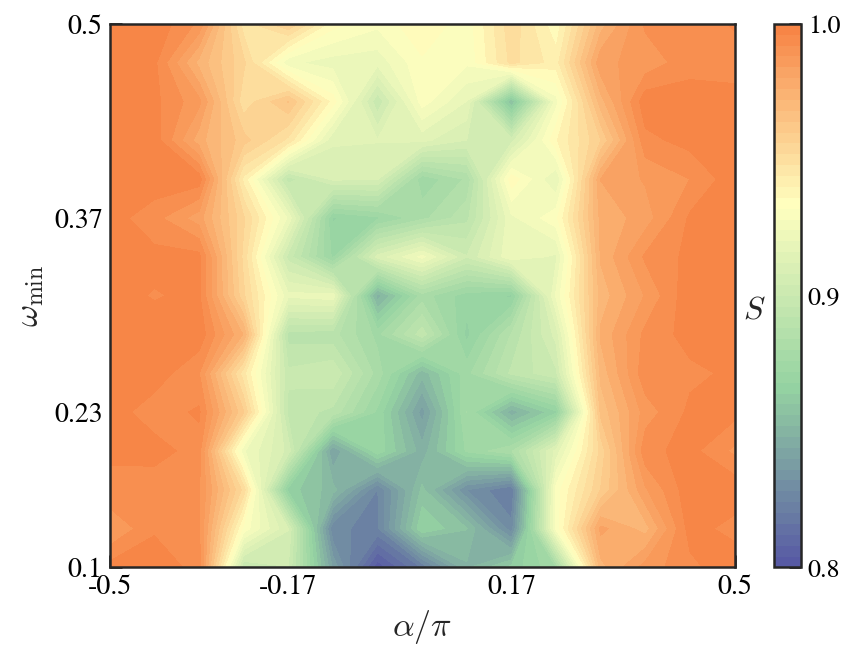
\includegraphics[width=1\textwidth]{figs/pd2.png}
        \caption{$\Delta \omega=2$}
        \label{fig:phaseDiagramDeltaOmega2}
    \end{subfigure}
    \caption{Phase diagrams of the system with different natural frequency differences $\Delta \omega$. The color represents the order parameter $S$ of the system.}
    \label{fig:phaseDiagrams}
\end{figure}

\begin{figure}[H]
    \centering
    \begin{subfigure}{0.45\textwidth}
        \centering
        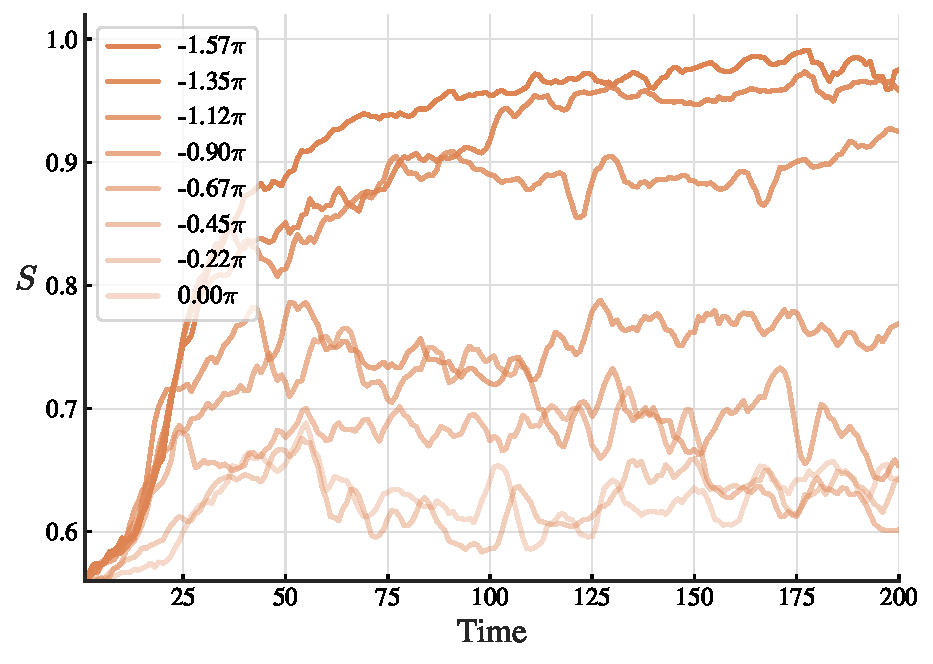
\includegraphics[width=1\textwidth]{figs/S_l0.15_d0.5_dO1_S.pdf}
        \caption{$\Delta \omega=1$}
        % \label{fig:phaseSeparation_singleChirality}
    \end{subfigure}
    \begin{subfigure}{0.45\textwidth}
        \centering
        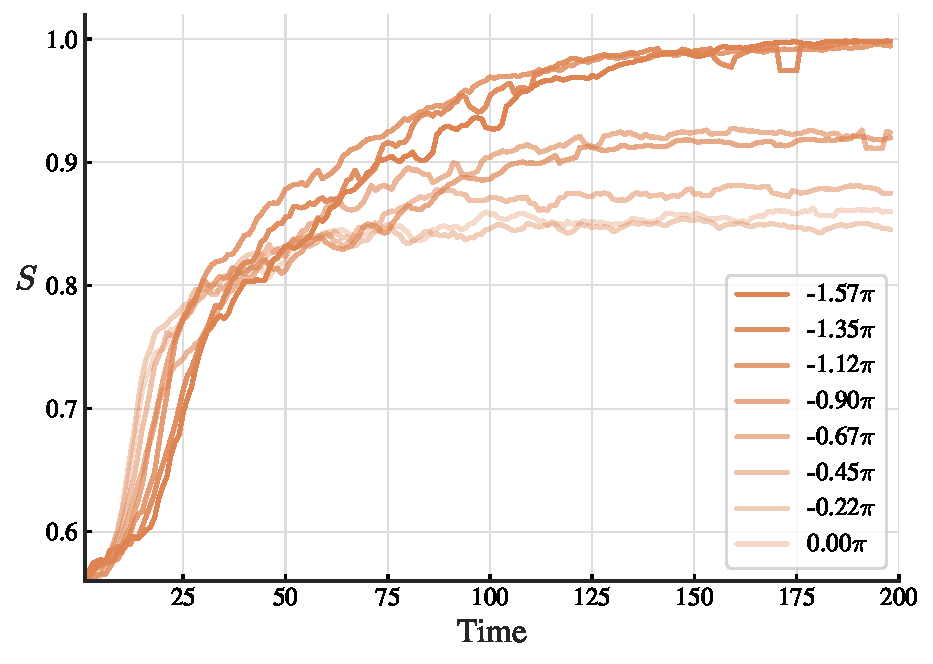
\includegraphics[width=1\textwidth]{figs/S_l0.15_d0.5_dO2_S.pdf}
        \caption{$\Delta \omega=2$}
        % \label{fig:phaseSeparation_doubleChirality}
    \end{subfigure}
    \caption{The order parameter $S$ v.s. time of the system with different natural frequency differences $\Delta \omega$ and $\omega_{\min}=0.1$}
    % \label{fig:phaseSeparation}
\end{figure}

\newpage
\section{Abstracted to a synchronization problem}
% \begin{figure}[H]
%     \centering
%     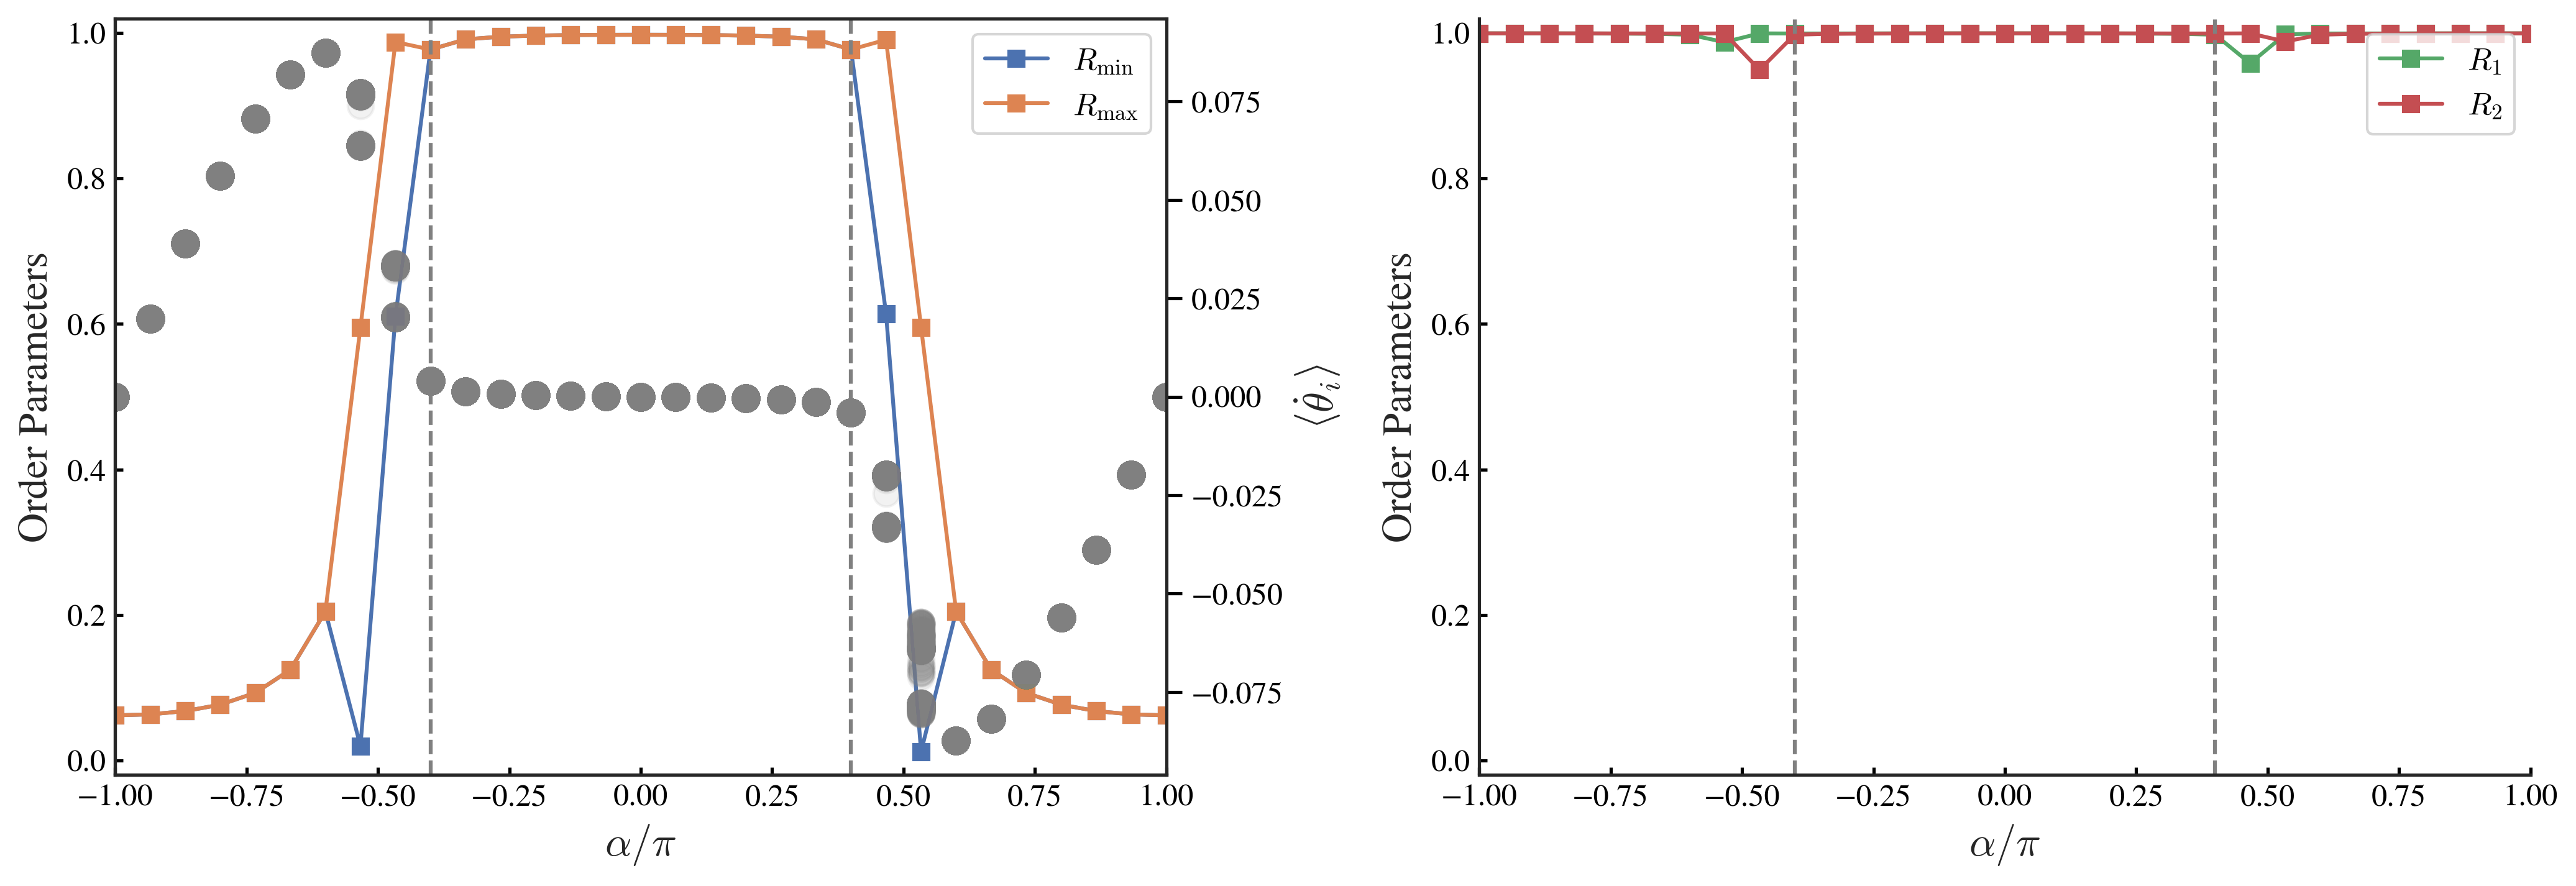
\includegraphics[width=1\textwidth]{figs/OrderParameter_R_l9.6_dO1.png}
%     \caption{The order parameter $R$ v.s. $\alpha_0$ and effective frequency $\left<\dot{\theta}_i\right>$ of the oscillator system with $\Delta \omega=1$ and $\omega_{\min}=0.1$}
% \end{figure}

The dynamics of the system (\ref{eq:totalDynamics}) in the ISS can be abstracted as a synchronization problem in multilayer networks. This problem can be described by the following equations:
\begin{equation}
    \label{eq:multiLayer}
    \begin{aligned}
        \dot{\theta}_{i}^{\pm}=&\omega _{i}^{\pm}+\frac{K}{N}\sum_{j=1}^{_{N^{\pm}}}{\sin \left( \theta _{j}^{\pm}-\theta _{i}^{\pm} \right)}\\
        &+\frac{K}{N}\sum_{j=1}^{_{N^{\mp}}}{\left[ \sin \left( \theta _{j}^{\mp}-\theta _{i}^{\pm}+\alpha _0 \right) -\sin \alpha _0 \right]}\;,
    \end{aligned}
\end{equation}
where $N^{\pm}=N/2$ is the numbers of swarmalators with positive and negative chirality, respectively. The first term in Eq.~(\ref{eq:multiLayer}) represents the intra-layer coupling between swarmalators with the same chirality, and the second term represents the inter-layer coupling between swarmalators with different chiralities. According to the definition of $g\left(\omega\right)$ in Eq.~(\ref{eq:lorentzian}), $\omega^{\pm}_i$ here follows the half-Lorentzian distribution:
\begin{equation}
    g^{+}\left( \omega \right) =\begin{cases}
        \frac{2}{\pi}\frac{\Delta}{\omega ^2+\Delta ^2},&		\omega \geqslant 0\\
        0,&		\mathrm{otherwise}\\
    \end{cases}
\end{equation}
and similarly for $g^{-}\left( \omega \right)$, replacing \enquote{$\omega \geqslant 0$} with \enquote{$< 0$}.

To quantify the inter-layer coherence of the system, it is convenient to define the generalized complex-valued
order parameters, i.e.,
\begin{equation}
    \label{eq:orderParameter}
    z_{n}^{\pm}\left( t \right) =r_{n}^{\pm}\left( t \right) \text{e}^{\text{i}\psi _{n}^{\pm}\left( t \right)}=\frac{1}{N}\sum_{j=1}^N{\text{e}^{\text{i}n\theta _{j}^{\pm}\left( t \right)}}\;,
\end{equation}
where $n=1,2,\dots, N$, and $r_{n}^{\pm}\left( t \right)$, $\psi _{n}^{\pm}\left( t \right)$ are the amplitudes and arguments of the $n$-order parameter.

% #####################################################
\begin{subequations}
    \begin{align}
        R_{\max}&=\max_{t\in \left[ T,T+h \right]} \left\{ R\left( t \right) \right\} 
        \\
        R_{\min}&=\min_{t\in \left[ T,T+h \right]} \left\{ R\left( t \right) \right\} 
    \end{align}
\end{subequations}

\begin{figure}[H]
    \centering
    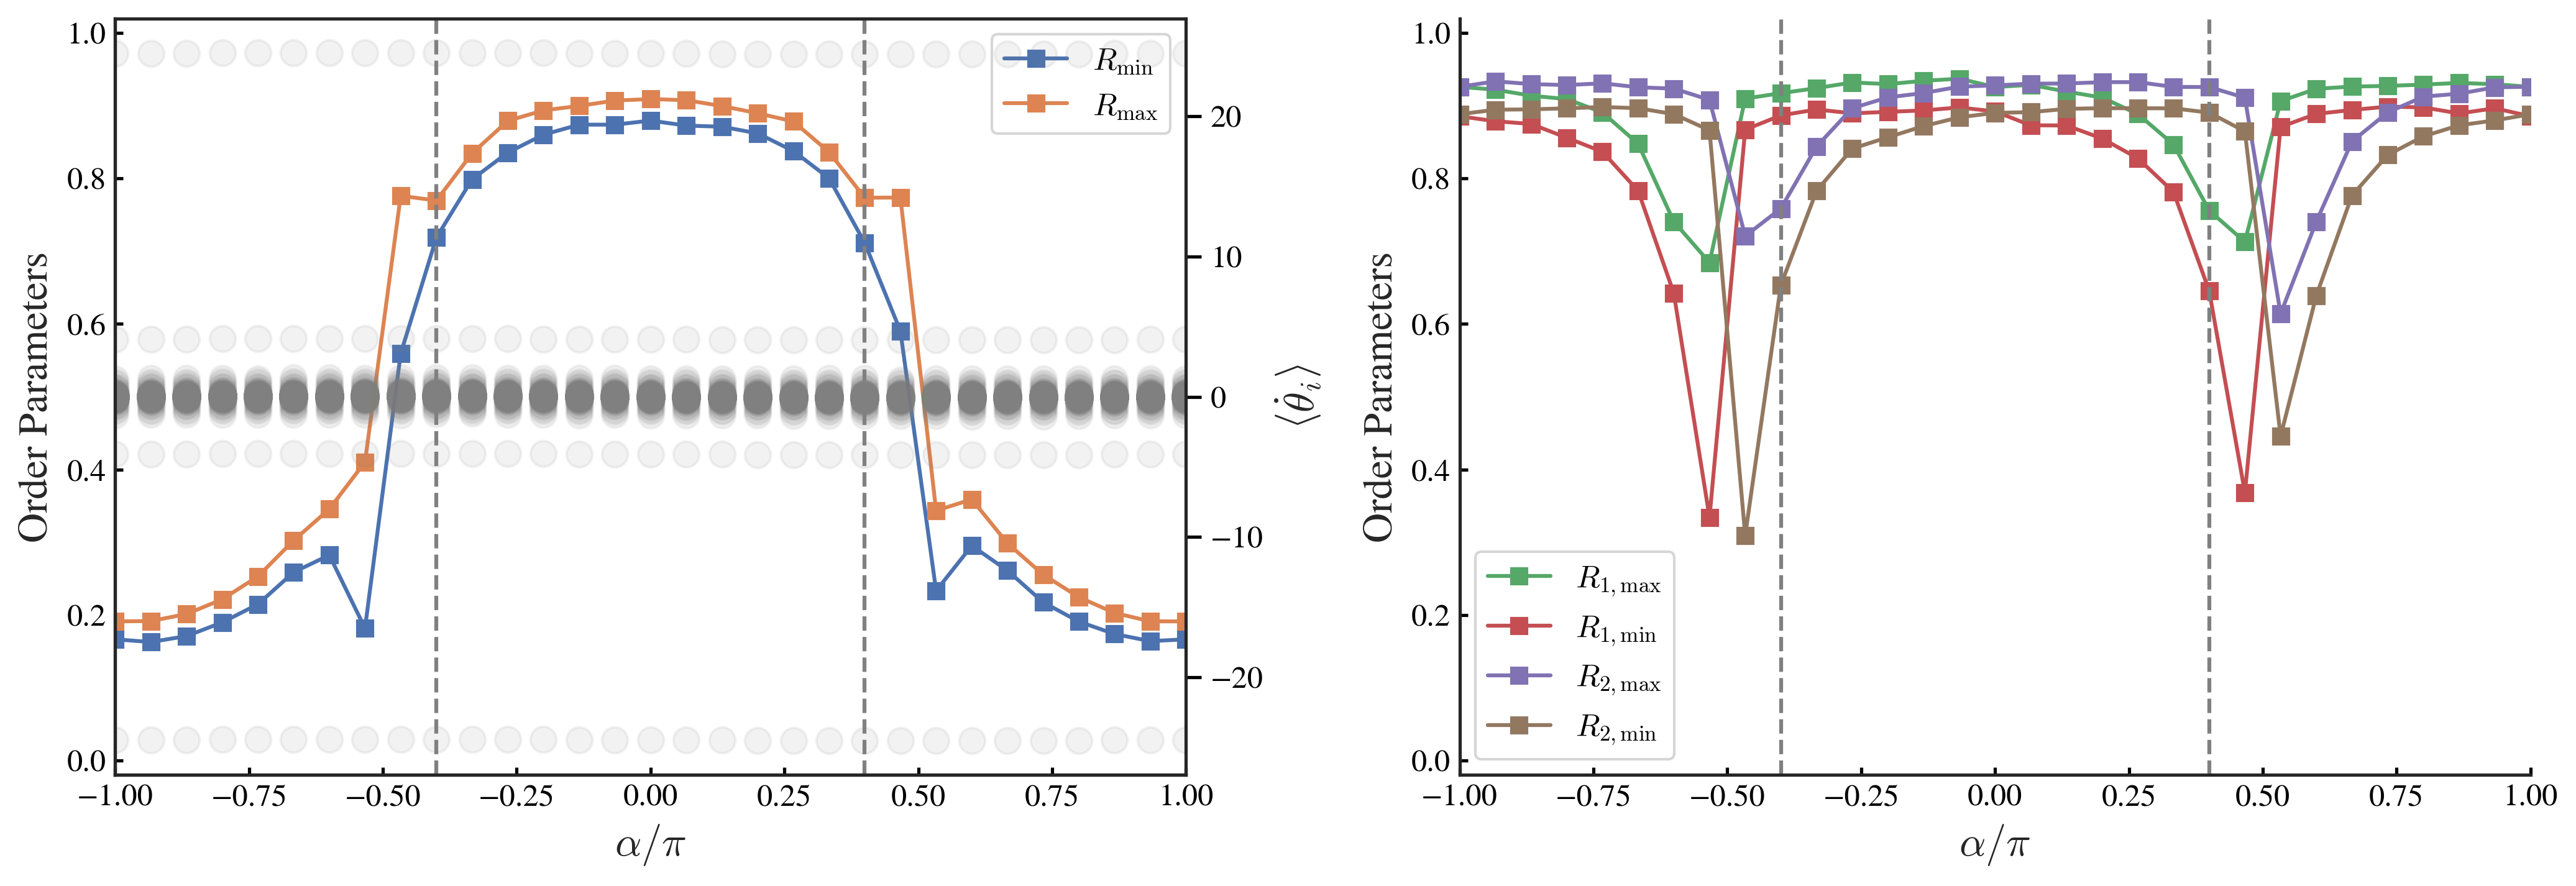
\includegraphics[width=1\textwidth]{figs/PurePhase_OrderParameter_R_l9.6_dO1.png}
    \caption{The order parameter $R$ v.s. $\alpha_0$ and effective frequency $\left<\dot{\theta}_i\right>$ of the oscillator system with $\Delta =1$}
\end{figure}

\begin{figure}[H]
    \centering
    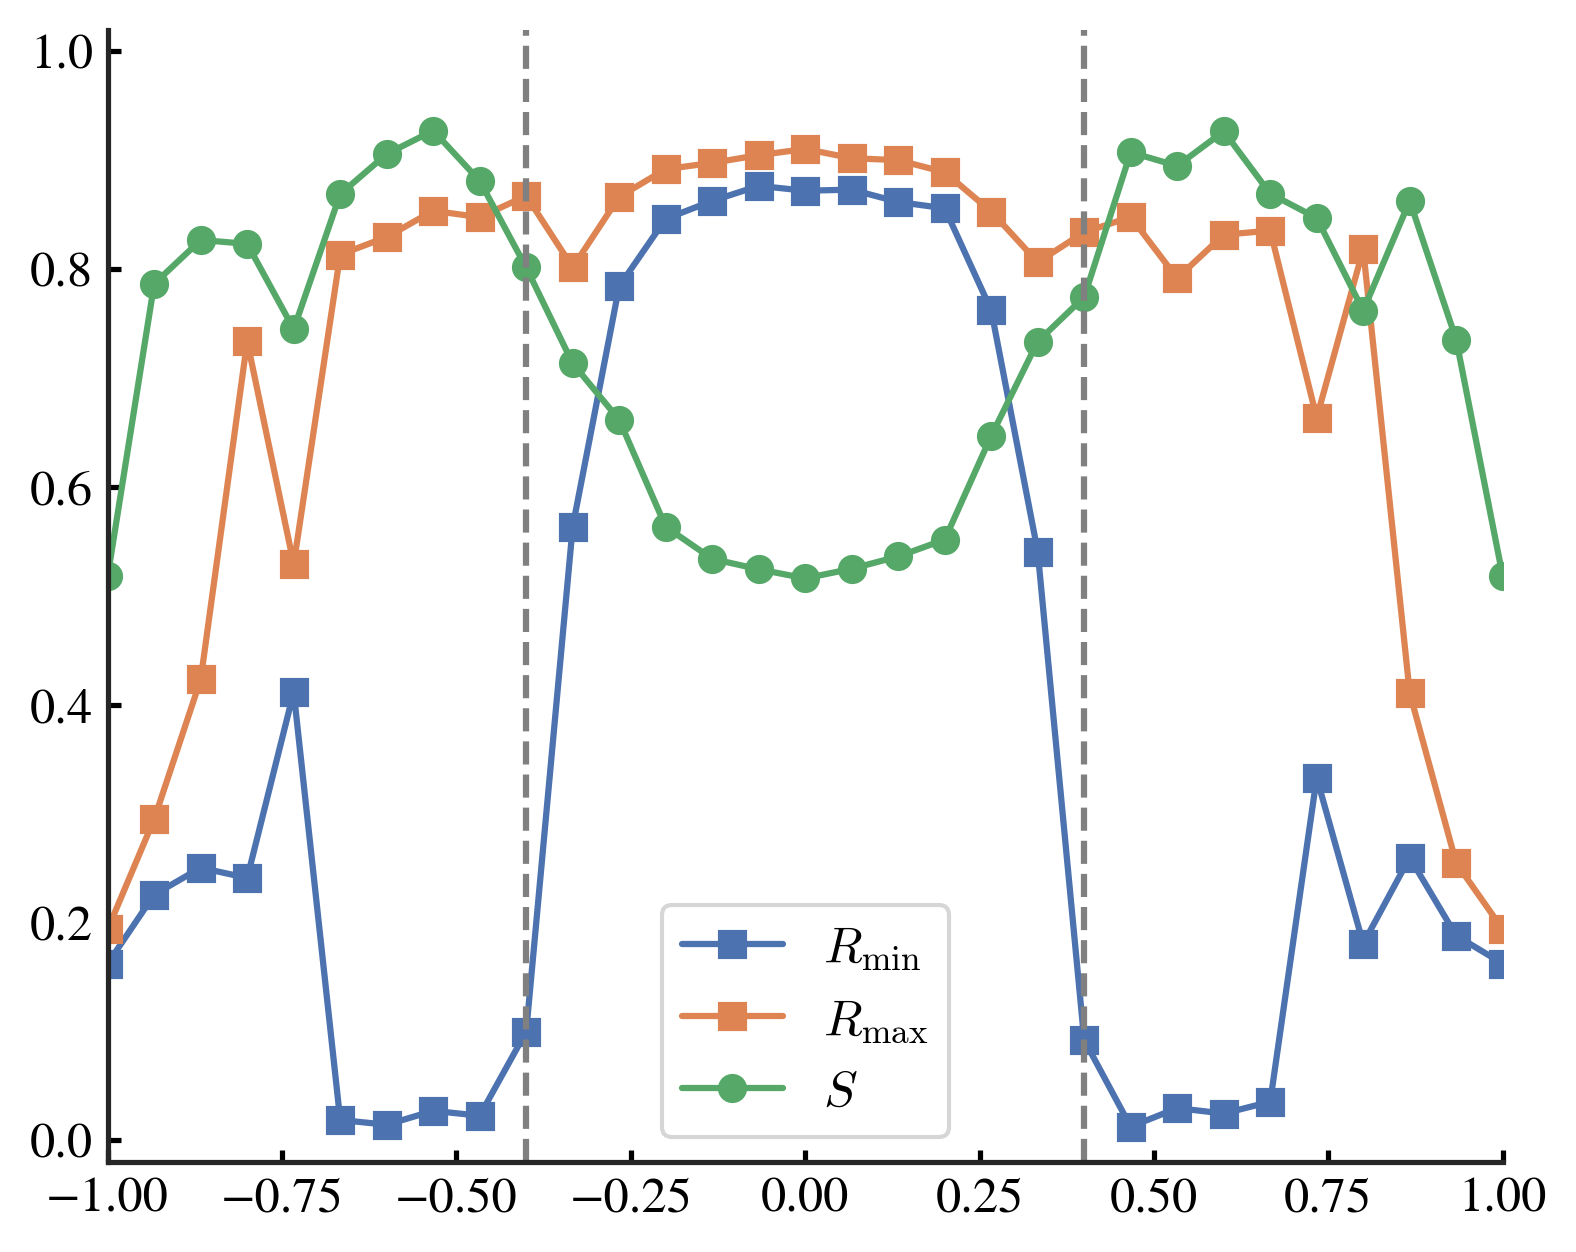
\includegraphics[width=0.45\textwidth]{figs/MeanFieldChiralInducedPhaseLag_OrderParameter_R_l9.6_d1_dO1_rS10.png}
    \caption{The order parameter $R$ v.s. $\alpha_0$ and effective frequency $\left<\dot{\theta}_i\right>$ of the swarmalator system with $\Delta =1$}
\end{figure}
% #####################################################

Our starting point is to analyze the critical point for the pulsation of the order parameter.
In the thermodynamic limit $N\rightarrow \infty$, where $N^{\pm}\rightarrow \infty$. Then
Eq.~(\ref{eq:multiLayer}) gives rise to the continuity equations
\begin{equation}
    \label{eq:continuity}
    \frac{\partial \rho ^{\pm}}{\partial t}+\frac{\partial}{\partial \theta}\left( \rho ^{\pm}v^{\pm} \right) =0
\end{equation}
where $\rho ^{\pm}\left( \theta ,\omega ,t \right)$ is the probability density of oscillators in layer $\pm$ with phase $\theta$ at fixed frequency $\omega$ and $t$, it satisfies the normalization condition
\begin{equation}
    \label{eq:normalization}
    \int_{0}^{2\pi}{\rho ^{\pm}\left( \theta ,\omega ,t \right) \text{d}\theta} =1\;.
\end{equation}
Here, $v^{\pm}\left( \theta ,\omega ,t \right)$ is the velocity field, given by
\begin{equation}
    \begin{aligned}
        &v^{\pm}\left( \theta ,\omega ,t \right) =\omega +\frac{K}{2}\sin \alpha _0\\
        &+\frac{K}{2}\int{\sin \left( \theta ^{\prime}-\theta \right) \rho ^{\pm}\left( \theta ^{\prime},\omega ^{\prime},t \right) \text{d}\theta ^{\prime}\text{d}\omega ^{\prime}}\\
        &+\frac{K}{2}\int{\sin \left( \theta ^{\prime}-\theta +\alpha _0 \right) \rho ^{\mp}\left( \theta ^{\prime},\omega ^{\prime},t \right) \text{d}\theta ^{\prime}\text{d}\omega ^{\prime}}\;.\\
    \end{aligned}
\end{equation}
Correspondingly, the 1-order parameter defined in Eq.~(\ref{eq:orderParameter}) in the thermodynamic limit reads
\begin{equation}
    \label{eq:continuityZ}
    z^{\pm}\left( t \right) =\int_{-\infty}^{+\infty}{g^{\pm}(\omega)\int_0^{2\pi}{\text{e}^{\text{i}\theta}\rho ^{\pm}\left( \theta ,\omega ,t \right) \text{d}\theta \text{d}\omega}}\;,
\end{equation}
then $v^{\pm}\left( \theta ,\omega ,t \right)$ simplifies to
\begin{equation}
v^{\pm}=\omega +\frac{K}{2}\sin \alpha _0+\frac{K}{2}\mathrm{Im}\left[ Z^{\pm}\left( t \right) \mathrm{e}^{-\mathrm{i}\theta} \right] 
\end{equation}
with the mean-field being
\begin{equation}
    Z^{\pm}\left( t \right) =z^{\pm}\left( t \right) +z^{\mp}\left( t \right) \mathrm{e}^{\mathrm{i}\alpha _0}
\end{equation}

To proceed, the probability $\rho ^{\pm}\left( \theta ,\omega ,t \right)$ can be expressed as a Fourier series of the following form
\begin{equation}
    \rho ^{\pm}\left( \theta ,\omega ,t \right) =\frac{1}{2\pi}\sum_{-\infty}^{+\infty}{a^{\pm} _n\left( \omega ,t \right) \mathrm{e}^{-\mathrm{i}n\theta}}\;,
\end{equation}
where $a^{\pm} _n\left( \omega ,t \right)$ is the $n$-th Fourier coefficient.

According to Ott and Antonsen ansatz \cite{10.1063/1.2930766, 10.1063/1.3136851}, the dynamics of the system can be reduced to a set of ordinary differential equations for the 1st Fourier coefficients $a^{\pm}\left( \omega ,t \right)$:
\begin{equation}
    \rho ^{\pm}=\frac{1}{2\pi}\left\{ 1+\sum_{n=1}^{\infty}{\left[ a^{\pm} \left( \omega ,t \right) \mathrm{e}^{-\mathrm{i}\theta} \right] ^n+\mathrm{c}.\mathrm{c}.} \right\} \;.
\end{equation}
To streamline the analysis, we express Eq.~(\ref{eq:continuity}) in its complex form by multiplying both sides by $\mathrm{e}^{\mathrm{i}\theta}$ and then integrating with respect to $\theta$:
\begin{equation}
    \label{eq:aDynamics}
    \begin{aligned}
        \dot{a}^{\pm}\left( \omega ,t \right) =&\mathrm{i}a^{\pm}\left( \omega ,t \right) \left( \omega +\frac{K}{2}\sin \alpha _0 \right)\\
        &+\frac{K}{4}\left[ Z^{\pm}\left( t \right) -\left( a^{\pm}\left( \omega ,t \right) \right) ^2\bar{Z}^{\pm}\left( t \right) \right] \;.
    \end{aligned}
\end{equation}
Herein, \enquote{$\bar{\cdot}$} denotes the complex conjugate.

To close the system, we express the complex order parameter $z^{\pm}\left( t \right)$ in Eq.~(\ref{eq:continuityZ}) by using Cauchy’s residue theorem with analytical continuation of $a^{\pm}\left( \omega ,t \right)$ into the right/left half complex plane for $g^{+}\left(\omega\right)$ and $g^{-}\left(\omega\right)$, respectively. Then we have
\begin{equation}
    \label{eq:zEqs2a}
    \begin{aligned}
        z^+\left( t \right) &=\int_0^{+\infty}{a^+\left( \omega ,t \right) g^+\left( \omega \right) \mathrm{d}\omega}\\
        &=\lim_{R\rightarrow \infty} \frac{1}{2}\int_{-\mathrm{i}R}^{\mathrm{i}R}{\frac{2}{\pi}\frac{\Delta a^+\left( \mathrm{i}\omega ,t \right)}{\left( \mathrm{i}\omega \right) ^2+\Delta ^2}\mathrm{d}\left( \mathrm{i}\omega \right)}\\
        &=a^+\left( \mathrm{i}\Delta ,t \right) \;,
    \end{aligned}
\end{equation}
and similarly, $z^-\left( t \right)=a^-\left( \mathrm{i}\Delta ,t \right)$.

As a result, the low-dimensional evolution of the order parameter can be obtained by letting $\omega =\mathrm{i}\Delta$ and substituting Eq.~(\ref{eq:zEqs2a}) into Eq.~(\ref{eq:aDynamics}), which yields
\begin{equation}
    \label{eq:zDynamics}
    \begin{aligned}
        \dot{z}^{\pm}=&z^{\pm}\left( \frac{\text{i}K}{2}\sin \alpha _0 - \Delta \right) +\frac{K}{4}\left( z^{\pm}+z^{\mp}\text{e}^{\text{i}\alpha _0} \right)-\frac{K}{4}\left( z^{\pm} \right) ^2\left( \bar{z}^{\pm}+\bar{z}^{\mp}\text{e}^{-\text{i}\alpha _0} \right) \;.\\
    \end{aligned}
\end{equation}
Then we rewrite the above equation using polar coordinates $z^{\pm}=r^{\pm}\mathrm{e}^{-\mathrm{i}\phi ^{\pm}}$. (The negative sign in the exponent is chosen to ensure that $\rho^{\pm}$ converges to $\delta\left(\theta-\phi^{\pm}\right)$, not $\delta\left(\theta+\phi^{\pm}\right)$ as $t\rightarrow\infty$.) Thus, $\phi^{\pm}$ can be interpreted as the phase of the chirality $\pm$, and $r^{\pm}$ measures the degree of synchronization of the chirality $\pm$. 
Then Eq.~(\ref{eq:zDynamics}) becomes
\begin{subequations}
    \small
    \begin{align}
        \dot{r}^{\pm}&=-r^{\pm}\Delta +K\frac{1 -\left( r^{\pm} \right) ^2}{4}\left[ r^{\pm}+r^{\mp}\cos \left( \phi ^{\pm}-\phi ^{\mp}+\alpha _0 \right) \right] ,\\
        \dot{\phi}^{\pm}&=-\frac{K}{2}\sin \alpha _0-Kr^{\mp}\frac{1+\left( r^{\pm} \right) ^2}{4r^{\pm}}\sin \left( \phi ^{\pm}-\phi ^{\mp}+\alpha _0 \right) .
    \end{align}
\end{subequations}
Introducing $\varphi=\phi^+-\phi^-$, the dynamics of the system can be further simplified to
\begin{subequations}
    \begin{align}
        \dot{r}^+=&-r^+\Delta +K\frac{1-\left( r^+ \right) ^2}{4}\left[ r^++r^-\cos \left( \varphi +\alpha _0 \right) \right] \;,\\
        \dot{r}^-=&-r^-\Delta +K\frac{1-\left( r^- \right) ^2}{4}\left[ r^-+r^+\cos \left( \varphi -\alpha _0 \right) \right] \;,\\
        \dot{\varphi}=&-Kr^-\frac{1+\left( r^+ \right) ^2}{4r^+}\sin \left( \varphi +\alpha _0 \right)-Kr^+\frac{1+\left( r^- \right) ^2}{4r^-}\sin \left( \varphi -\alpha _0 \right)
    \end{align}
\end{subequations}

\section{\label{sec:analysis}Coarse grained equations and phase diagrams}

We begin with Eq.~(\ref{eq:totalDynamics}), replacing the finite coupling distance alignment interaction with a pseudopotential (the '$\delta$'-interaction). This substitution is justified when the interaction is sufficiently short-ranged, making the specific shape of the associated interaction potential irrelevant to the dynamics of many swarmalators. The pseudopotential is defined as:
\begin{subequations}
    \begin{align}
        &\dot{\mathbf{r}}_{i}^{\pm}=v\mathbf{p}\left( \theta _{i}^{c} \right) \;,\\
        &\dot{\theta}_{i}^{\pm}=\omega _{i}^{\pm}+K\sum_{j=1}{\left\{ \delta \left( \mathbf{r}_{j}^{\pm}-\mathbf{r}_{i}^{\pm} \right) \sin \left( \theta _{j}^{\pm}-\theta _{i}^{\pm} \right) \right.}\notag\\
        &\left. +\delta \left( \mathbf{r}_{j}^{\mp}-\mathbf{r}_{i}^{\pm} \right) \left[ \sin \left( \theta _{j}^{\mp}-\theta _{i}^{\pm}+\alpha _0 \right) -\sin \alpha _0 \right] \right\} \;,
    \end{align}
\end{subequations}
where $c\in\left\{+,-\right\}$ is the chirality of the swarmalator $i$ and $b=+$ if $c=-$ and vice versa.  
Then following \cite{David_S_Dean_1996} we derive a continuum equation of motion for the combined $N$-swarmalator probability density
\begin{equation}
    \label{eq:globalContinuityDef}
    \rho ^{\pm}\left( \mathbf{r},\theta ,t \right) =\sum_{i=1}{\rho _{i}^{\pm}\left( \mathbf{r},\theta ,t \right)}\;,
\end{equation}
where $\rho _{i}^{\pm}\left( \mathbf{r},\theta ,t \right) =\delta \left( \mathbf{r}_{i}^{\pm}\left( t \right) -\mathbf{r} \right) \delta \left( \theta _{i}^{\pm}\left( t \right) -\theta \right)$ is the probability density of finding $i$-th swarmalator at position $\mathbf{r}$ with phase $\theta$ and chirality $+$ or $-$ at time $t$.
Since the deterministic dynamical equation Eq.~ (\ref{eq:totalDynamics}) conserves the number of oscillators with a given natural frequency over time, the distribution function evolves according to a continuity equation of the following form:
\begin{equation}
    \frac{\partial \rho _{i}^{\pm}}{\partial t}=-\nabla \cdot \left( \rho _{i}^{\pm}v_{\mathbf{r}} \right) -\frac{\partial}{\partial \theta}\left( \rho _{i}^{\pm}v_{\theta}^{\pm ,i} \right) \;.
    \label{eq:singleContinuity}
\end{equation}
Here, the velocity fields read
\begin{subequations}
    \begin{align}
        &v_{\mathbf{r}}\left( \mathbf{r},\theta ,t \right) =v\mathbf{p}\left( \theta \right) \;,\\
        &v_{\theta}^{\pm ,i}\left( \mathbf{r},\theta ,t \right) =\omega _{i}^{\pm}+K\int_{-\pi}^{\pi}{\mathrm{d}\phi \left\{ \rho ^{\pm}\left( \mathbf{r},\phi ,t \right) \sin \left( \phi -\theta \right) \right.}\notag\\
        &\left. +\rho ^{\mp}\left( \mathbf{r},\phi ,t \right) \left[ \sin \left( \phi -\theta +\alpha _0 \right) -\sin \alpha _0 \right] \right\} \;.
    \end{align}
\end{subequations}
Summing Eq.~(\ref{eq:singleContinuity}) over the $i$ and $\pm$ indices, and using the definition of the density $\rho ^\pm$ in Eq.~(\ref{eq:globalContinuityDef}), we obtain  
\begin{equation}
    \label{eq:globalContinuity}
    \begin{aligned}
        &\frac{\partial}{\partial t}\rho ^{\pm}\left( \mathbf{r},\theta ,t \right) =-v\mathbf{p}\left( \theta \right) \cdot \nabla \rho ^{\pm}\left( \mathbf{r},\theta ,t \right) -\frac{\partial}{\partial \theta}\Omega^{\pm}\\
        &-K\frac{\partial}{\partial \theta}\rho ^{\pm}\left( \mathbf{r},\theta ,t \right) \int_{-\pi}^{\pi}{\mathrm{d}\phi}\left\{ \rho ^{\pm}\left( \mathbf{r},\phi ,t \right) \sin \left( \phi -\theta \right) \right.\\
        &\left. +\rho ^{\mp}\left( \mathbf{r},\phi ,t \right) \left[ \sin \left( \phi -\theta +\alpha _0 \right) -\sin \alpha _0 \right] \right\} \;,\\
    \end{aligned}
\end{equation}
where $\Omega^{\pm} \left( \mathbf{r},\theta ,t \right) =\sum_{i=1}{\rho _{i}^{\pm}\left( \mathbf{r},\theta ,t \right) \omega _{i}^{\pm}}$.
Spatial homogeneity and phase synchronization of the ISS indicates
 $\forall i$, $\rho _{i}^{\pm}\left( \mathbf{r},\theta ,t \right) \equiv \rho _{\text{ISS}}\left( \mathbf{r},\theta ,t \right)$, which yields
\begin{equation}
    \Omega ^{\pm}\left( \mathbf{r},\theta ,t \right) =\rho ^{\pm}\left( \mathbf{r},\theta ,t \right) \bar{\omega}^{\pm}\;,
\end{equation} 
where $\bar{\omega}^{\pm}=\left< \omega _{i}^{\pm} \right>$.

Transforming $\rho^{\pm}$ in a Fourier series in $\theta$, we have 
\begin{equation}
    \rho ^{\pm}\left( \mathbf{r},\theta ,t \right) =\frac{1}{2\pi}\sum_{k=-\infty}^{+\infty}{\varrho _{k}^{\pm}\left( \mathbf{r},t \right)}\mathrm{e}^{-\mathrm{i}k\theta}\;,
\end{equation}
where $\varrho _{k}^{\pm}$ is the $k$-th Fourier coefficient of $\rho^{\pm}$, defined as
\begin{equation}
    \varrho _{k}^{\pm}\left( \mathbf{r},t \right) =\int{\rho ^{\pm}\left( \mathbf{r},\theta ,t \right) \text{e}^{\text{i}k\theta}\text{d}\theta}\;.
\end{equation}
To streamline the analysis, we express Eq.~(\ref{eq:globalContinuity}) in its complex form by multiplying both sides by $\mathrm{e}^{\mathrm{i}k\theta}$ and then integrating with respect to $\theta$:
\begin{equation}
    \label{eq:hierarchyEqs}
    \begin{aligned}
        \dot{\varrho}_{k}^{\pm}&=-\frac{v}{2}\left[ \partial _x\left( \varrho _{k+1}^{\pm}+\varrho _{k-1}^{\pm} \right) -\mathrm{i}\partial _y\left( \varrho _{k+1}^{\pm}-\varrho _{k-1}^{\pm} \right) \right]\\
        &+\mathrm{i}k\bar{\omega}^{\pm}\varrho _{k}^{\pm}\\
        &+\frac{\mathrm{i}kK}{2\pi}\sum_{m=-\infty}^{\infty}{\varrho _{k-m}^{\pm}F_{-m}\varrho _{m}^{\pm}}\\
        &+\frac{\mathrm{i}kK}{2\pi}\sum_{m=-\infty}^{\infty}{\mathrm{e}^{\mathrm{i}m\alpha _0}\varrho _{k-m}^{\pm}F_{-m}\varrho _{m}^{\mp}}\\
        &-\mathrm{i}kK\varrho _{0}^{\mp}\varrho _{k}^{\pm}\sin \alpha _0\;,
    \end{aligned}
\end{equation}
where $F_m$ is the $m$-th Fourier coefficient of $\sin \theta$. Evaluating Eq.~(\ref{eq:hierarchyEqs}) for $k=0, 1, \dots$ leads to a hierarchy of equations for $\left\{\varrho_k^{\pm}\right\}$ with 
\begin{equation}
    \rho^{\pm} \left(\mathbf{r}, t\right)=\varrho_0^{\pm}\left(\mathbf{r}, t\right) = \int_{-\pi}^{\pi}{\rho^{\pm}\left(\mathbf{r}, \theta, t\right)\mathrm{d}\theta}
\end{equation}
being the probability density of finding a swarmalator at position $\mathbf{r}$ at time $t$ and 
\begin{equation}
    \mathbf{w}^{\pm}\left( \mathbf{r},t \right) =\left( \mathrm{Re}\varrho _1^{\pm},\mathrm{Im}\varrho _1^{\pm} \right) =\int_{-\pi}^{\pi}{\mathbf{p}\left( \theta \right) \rho^{\pm} \left( \mathbf{r},\theta ,t \right) \mathrm{d}\theta}
\end{equation}
being the momentum field at position $\mathbf{r}$ at time $t$.
The degree modulus $R^{\pm}\left( \mathbf{r},t \right) =\left| \mathbf{w}^{\pm}\left( \mathbf{r},t \right) \right|$ is the absolute value of the mean normalized velocity of local swarmalators, which can be used as a measure of the local degree of synchronization. 

To close the hierarchy of equations Eq.~(\ref{eq:hierarchyEqs}), we truncate the series at a finite order $K$ and neglect the higher-order terms. This truncation is justified when the interaction is sufficiently short-ranged, making the specific shape of the associated interaction potential irrelevant to the dynamics of many swarmalators. Specifically, we assume that $\varrho_2^{\pm}\left(\mathbf{r},t\right)$ follows changes in $\varrho_0^{\pm}\left(\mathbf{r},t\right)$ and $\varrho_1^{\pm}\left(\mathbf{r},t\right)$ adiabatically ($\dot{\varrho}_2^{\pm}\left( \mathbf{r},t \right) \approx 0$) and neglect the higher-order terms ($\varrho _{k\geqslant 3}^{\pm}\left( \mathbf{r},t \right) \approx 0$).
% For $k=0$, Eq.~(\ref{eq:hierarchyEqs}) gives the continuity equation
% \begin{equation}
%     \dot{\rho}^{\pm}=\dot{\varrho}_{0}^{\pm}=-v\left( \partial _x\mathrm{Re}\varrho _{1}^{\pm}+\partial _y\mathrm{Im}\varrho _{1}^{\pm} \right) =-v\nabla \cdot \mathbf{w} \;.
% \end{equation}
Truncating at order 3, we are left with
\begin{subequations}
    \begin{align}
        &\dot{\varrho}_{0}^{\pm}=-\mathrm{Re}\bar{\nabla}\varrho _{1}^{\pm}\\
        &\dot{\varrho}_{1}^{\pm}=-\frac{v}{2}\left( \nabla \varrho _{0}^{\pm}+\bar{\nabla}\varrho _{2}^{\pm} \right)+\mathrm{i}\varrho _{1}^{\pm}\left( \bar{\omega}^{\pm}-K\varrho _{0}^{\mp}\sin \alpha _0 \right)\notag\\
        &+\frac{K}{2}\varrho _{0}^{\pm}\left( \varrho _{1}^{\pm}+\mathrm{e}^{\mathrm{i}\alpha _0}\varrho _{1}^{\mp} \right) \;,\label{eq:secondOrder}\\
        &\dot{\varrho}_{2}^{\pm}=-\frac{v}{2}\nabla \varrho _{1}^{\pm}+\mathrm{i}2\varrho _{k}^{\pm}\left( \bar{\omega}^{\pm}-K\varrho _{0}^{\mp}\sin \alpha _0 \right)\notag\\
	    &+K\varrho _{1}^{\pm}\left( \varrho _{1}^{\pm}+\mathrm{e}^{\mathrm{i}\alpha _0}\varrho _{1}^{\mp} \right)\;,\label{eq:thirdOrder}
    \end{align}
\end{subequations}
where $\nabla =\partial _x+\mathrm{i}\partial _y$ denotes the gradient operator in the complex plane, and $\bar{\nabla}=\partial _x-\mathrm{i}\partial _y$ is the complex conjugate of $\nabla$. Let $\dot{\varrho}_2^{\pm}=0$, then $\varrho_2^{\pm}$ can be solved as
\begin{equation}
    \varrho _{2}^{\pm}=-\frac{\mathrm{i}K\varrho _{1}^{\pm}}{a^{\pm}}\left( \varrho _{1}^{\pm}+\mathrm{e}^{-\mathrm{i}\alpha _0}\varrho _{1}^{\mp} \right) +\frac{\mathrm{i}\nabla \varrho _{1}^{\pm}v}{2a^{\pm}}
\end{equation}
where $a^{\pm}=2\left( K\rho ^{\mp}\sin \alpha _0-\bar{\omega}^{\pm} \right) $. Substituting $\varrho_2^{\pm}$ into Eq.~(\ref{eq:secondOrder}), we have
\begin{equation}
    \begin{aligned}
        \dot{\varrho}_{1}^{\pm}&=-\frac{v}{2}\nabla \varrho _{0}^{\pm}+\frac{\mathrm{i}vK\bar{\nabla}\varrho _{1}^{\pm}}{2a^{\pm}}\left( \varrho _{1}^{\pm}+\mathrm{e}^{-\mathrm{i}\alpha _0}\varrho _{1}^{\mp} \right)\\
        &+\frac{\mathrm{i}vK\varrho _{1}^{\pm}}{2a^{\pm}}\left( \bar{\nabla}\varrho _{1}^{\pm}+\mathrm{e}^{-\mathrm{i}\alpha _0}\bar{\nabla}\varrho _{1}^{\mp} \right) -\frac{\mathrm{i}v^2\Delta \varrho _{1}^{\pm}}{4a^{\pm}}\\
        &+\mathrm{i}\varrho _{1}^{\pm}\left( \bar{\omega}^{\pm}-K\varrho _{0}^{\mp}\sin \alpha _0 \right) +\\
        &\frac{K}{2}\varrho _{0}^{\pm}\left( \varrho _{1}^{\pm}+\mathrm{e}^{\mathrm{i}\alpha _0}\varrho _{1}^{\mp} \right)\\
    \end{aligned}
\end{equation}

\bibliography{ref}

\end{document}